\section{Synthetic-data fidelity}\label{sec:fidelity}

A null augmentation result is only informative if the generator itself worked. Every metric
below compares synthetic rows against the real training rows \emph{of the same fold}, never
the test papers (Table~\ref{tab:fidelity}, Fig.~\ref{fig:fid}).

\paragraph{Marginals.} The mean Kolmogorov--Smirnov statistic is
0.154 and \textbf{no} continuous variable was rejected at
$p<0.05$ in any fold, ratio or seed.

\paragraph{Categorical frequencies.} The mean Jensen--Shannon distance is
0.079, indicating close agreement of level frequencies.

\paragraph{Dependency structure.} The Pearson correlation matrix differs by
0.047 in mean absolute value and the normalised
mutual-information matrix, which also covers the categorical descriptors, by
0.055.

\paragraph{Descriptor--target relationships.} This is the fidelity criterion that matters
most for downstream utility, since a generator can match every marginal and still destroy the
relationship a regressor must learn. Measured as Spearman correlation with the target for
continuous descriptors and $\eta^2$ for categorical ones, the mean absolute change is
0.065.

\paragraph{Memorisation.} Across all folds, ratios and seeds,
0 synthetic rows were exact copies of a real
training row and 0 were duplicated within a
synthetic set. The median synthetic-to-real nearest-neighbour distance is
0.33 times the median
real-to-real distance. A ratio below unity is expected rather than alarming here, since
37--200 synthetic points are drawn
over the same manifold as 37 real ones and
nearest-neighbour distances contract with density alone; the sharper diagnostic is that only
3.5 of
116 synthetic rows on average fall closer to a real record than
the fifth percentile of real-to-real spacing.

\paragraph{Central interpretation.} The generator reproduced the joint distribution it was
shown, and did so without copying. \textbf{Distributional fidelity to the training fold does
not imply improved generalisation to a held-out publication.} A Bayesian network resamples
the dependencies present in its training data; it cannot supply information about
experimental domains the training papers never visited. Since Sec.~\ref{sec:domainshift}
establishes that the held-out papers are precisely such unvisited domains, the null result of
Sec.~\ref{sec:augres} is the expected outcome rather than an anomaly, and it is not
attributable to a defective generator.

\begin{figure*}[htbp]\centering
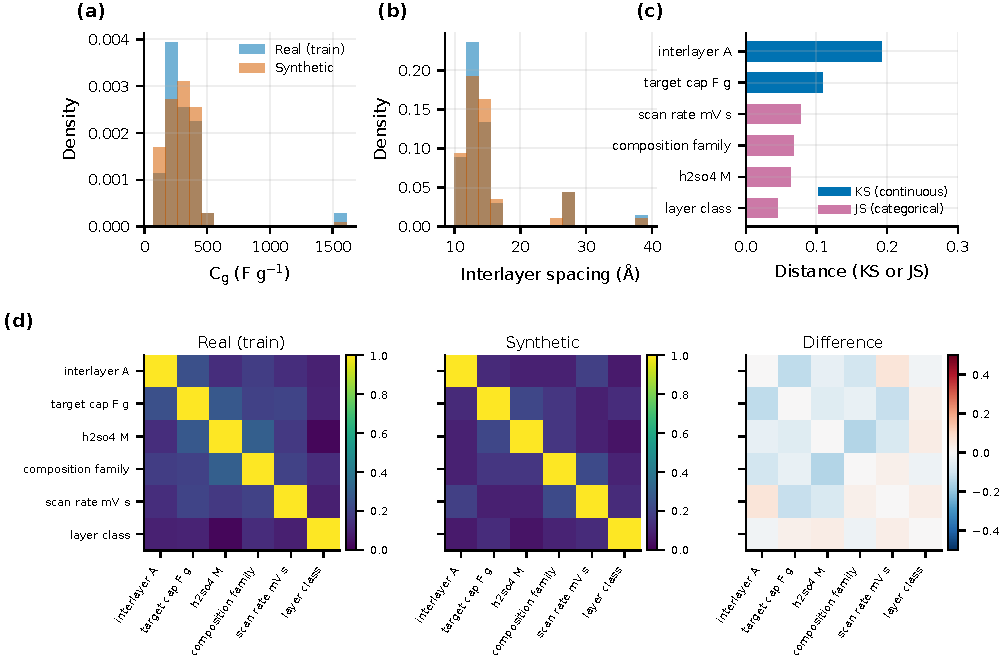
\includegraphics[width=\textwidth]{figures/fig04_synthetic_fidelity.pdf}
\caption{Fidelity of the Bayesian-resampled observations against the real training rows of
the same fold. (a) Target marginal, (b) interlayer-spacing marginal, (c) per-variable
Kolmogorov--Smirnov (continuous) and Jensen--Shannon (categorical) distances, (d) normalised
mutual-information matrices for real and synthetic data and their difference.}
\label{fig:fid}\end{figure*}

\begin{table}[htbp]
\centering
\caption{Fidelity of the Bayesian-network synthetic observations, computed against the real training rows of the same fold ($k=2$; mean, min and max over folds, augmentation ratios and generator seeds).}
\label{tab:fidelity}
\footnotesize
\begin{tabular}{lrrr}
\toprule
\textbf{Fidelity metric} & \textbf{Mean} & \textbf{Min} & \textbf{Max} \\
\midrule
Mean KS statistic (continuous) & 0.154 & 0.095 & 0.198 \\
Continuous variables with KS $p<0.05$ & 0.0 & 0.0 & 0.0 \\
Mean Jensen--Shannon distance (categorical) & 0.079 & 0.028 & 0.170 \\
Pearson correlation matrix, mean $|\Delta|$ & 0.047 & 0.002 & 0.346 \\
Spearman correlation matrix, mean $|\Delta|$ & 0.095 & 0.001 & 0.292 \\
Mutual-information matrix, mean $|\Delta|$ & 0.055 & 0.025 & 0.093 \\
Descriptor--target association, mean $|\Delta|$ & 0.065 & 0.010 & 0.263 \\
Exact duplicates of a real training row & 0.0 & 0.0 & 0.0 \\
Duplicates within a synthetic set & 0.0 & 0.0 & 0.0 \\
Synthetic$\rightarrow$real NN distance (median) & 0.0065 & 0.0046 & 0.0086 \\
Real$\rightarrow$real NN distance (median) & 0.0195 & 0.0130 & 0.0351 \\
\bottomrule
\end{tabular}
\par\vspace{2pt}\begin{minipage}{\linewidth}\scriptsize Nearest-neighbour distances use a range-normalised mixed-type (Gower) metric. No synthetic row reproduced a real training row exactly.\end{minipage}
\end{table}
